\section{Use case: investigation of the noise impact on Auto Encoder algorithm}\label{usecase}
This section presents a complete case study that constructs artificial noise experiments to quantitatively evaluate the effects of three typical noise types-Gaussian noise, drift, and spikes—on the trajectory reconstruction performance of an AE model. The results further help to identify key priorities and directions for the data cleaning stage.
The experiment employs an ADS-B dataset collected at Zurich Airport, covering trajectory data recorded from 04:57:13 (UTC) on October 1, 2019 to 18:57:37 (UTC) on November 30, 2019, as shown in Figure \ref{fig:totaltracks}. The dataset contains approximately 2.8 million ADS-B messages, representing the complete trajectories of about 14,000 flights. Each record includes fields such as timestamp, altitude, longitude, latitude, ground speed, heading, callsign, and ICAO24 code, with longitude ranging from 7.5702 to 9.5276 and latitude from 46.8019 to 48.1302.
\begin{figure}[h]
	\centering
	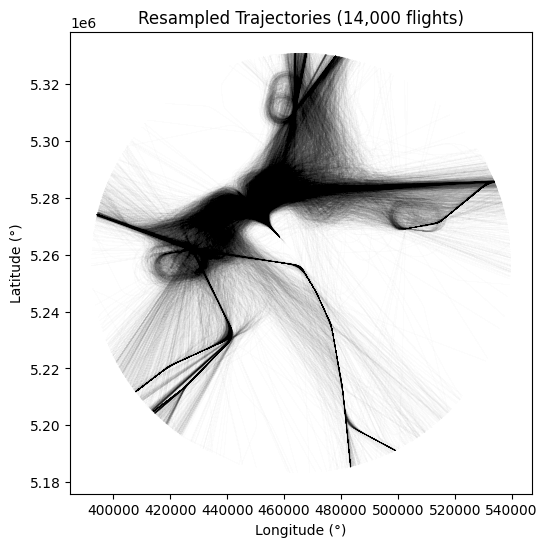
\includegraphics[height=5cm]{totaltracks}
	\caption{Visualization of All Flight Trajectories at Zurich Airport from 04:57:13 on October 1, 2019 to 18:57:37 on November 30, 2019: Resampled Trajectories (14,000 Flights) with Transparency to Reflect Trajectory Distribution Density}
	\label{fig:totaltracks}
\end{figure}

For model training, the data were preprocessed as follows: trajectories were resampled so that each one contained 100 coordinate points, ensuring a uniform input dimension; and normalization was applied to preserve the spatial proportion of coordinates.

\subsection{Auto-encoder Model}
In terms of algorithm selection, this study builds a simple yet stable AE model. The AE learns the latent space representation of flight trajectories by performing unsupervised feature compression and reconstruction, enabling it to reproduce the input trajectory data.
The AE comprises two symmetric subnetworks: an encoder and a decoder. The encoder compresses a 200-dimensional trajectory vector through layers of 128, 64, and 32 neurons into a 32-dimensional latent representation. The decoder mirrors this structure to reconstruct the trajectory back to 200 dimensions.

The dataset is divided into training and validation sets (8:2), and the AE is trained unsupervised under consistent normalization. Training and validation losses are monitored for convergence, which occurs after about 200 epochs with $\mathrm{MSE} \approx 0.002$, indicating effective learning and strong reconstruction performance.

\subsection{Baseline Generation}
The trained AE model identifies trajectories most similar to clean data as the baseline. It reconstructs all normalized samples and ranks them by reconstruction error, selecting those with the lowest errors.
Trajectories that are highly reconstructable, which show minimal error, are considered the most representative and clean within the dataset.
As shown in Figure \ref{fig:best100}, the baseline trajectories exhibit high smoothness and spatial consistency, conforming to the physical laws of real flight paths. In contrast, high-error samples, showed in Figure \ref{fig:worst100}, often contain data anomalies or noisy points.
Using AE reconstruction error as the selection criterion enables automatic identification of high-quality trajectories without manual thresholds or interpolation. This method helps avoid errors or inappropriate parameter settings that can arise during manual preprocessing, thereby producing a statistically sound and model-adaptive baseline dataset. In total, 100 high-quality trajectories were selected as the baseline dataset for the experiment.

%\begin{figure}[h]
%	\centering
%	\begin{subfigure}[t]{0.4\textwidth}
%		\centering
%		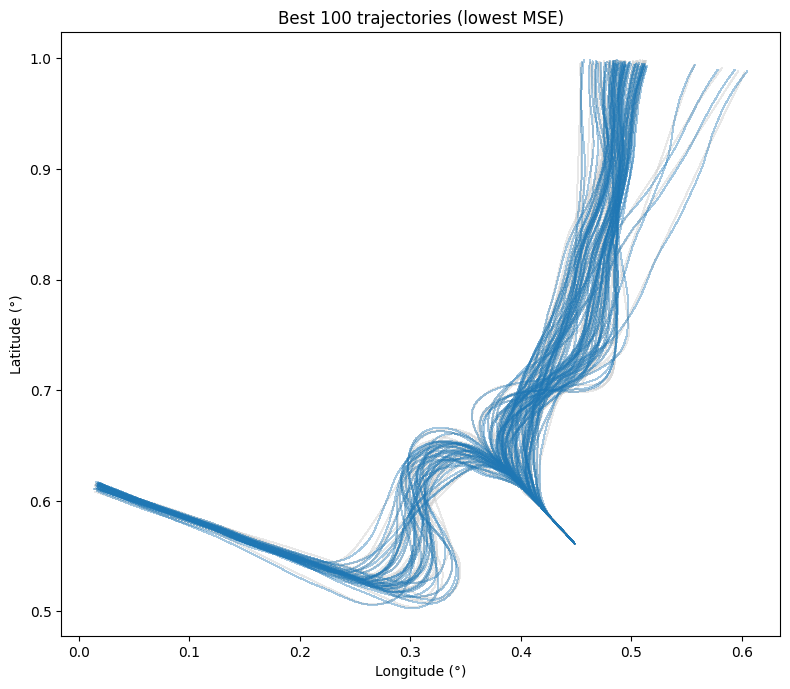
\includegraphics[height=4cm]{best100}
%		\caption{The best 100 trajectories}  
%		\label{fig:best100}  
%	\end{subfigure}
%\hspace{0.05\textwidth}	
%\begin{subfigure}[t]{0.45\textwidth}
%	\centering
%	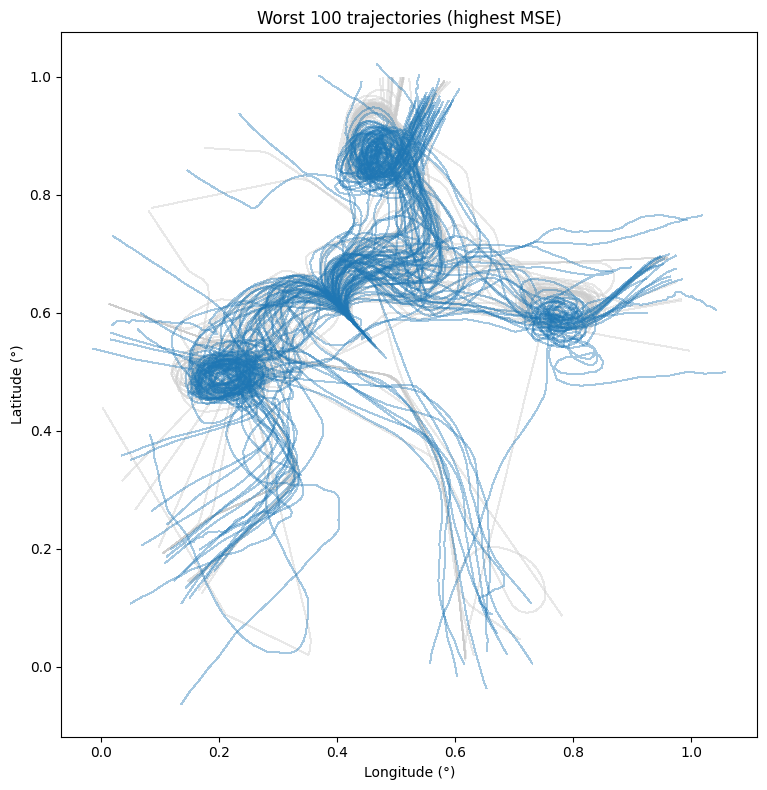
\includegraphics[height=4cm]{worst100}
%	\caption{The worst 100 trajectories}  
%	\label{fig:worst100}
%\end{subfigure}
%\caption{Visualization of Trajectory Reconstruction Results by Trained AE Model: (a) The Best 100 Trajectories with the Lowest MSE, and (b) The Worst 100 Trajectories with the Highest MSE}
%\label{conparison of best and worst}
%\end{figure}

\begin{figure}[htbp]
	\centering
	\begin{floatrow}
		% --- 左图 ---
		\ffigbox
		[% 指定 float box 的宽度(与图宽相同)
		0.45\textwidth
		]
		{% 图片内容
			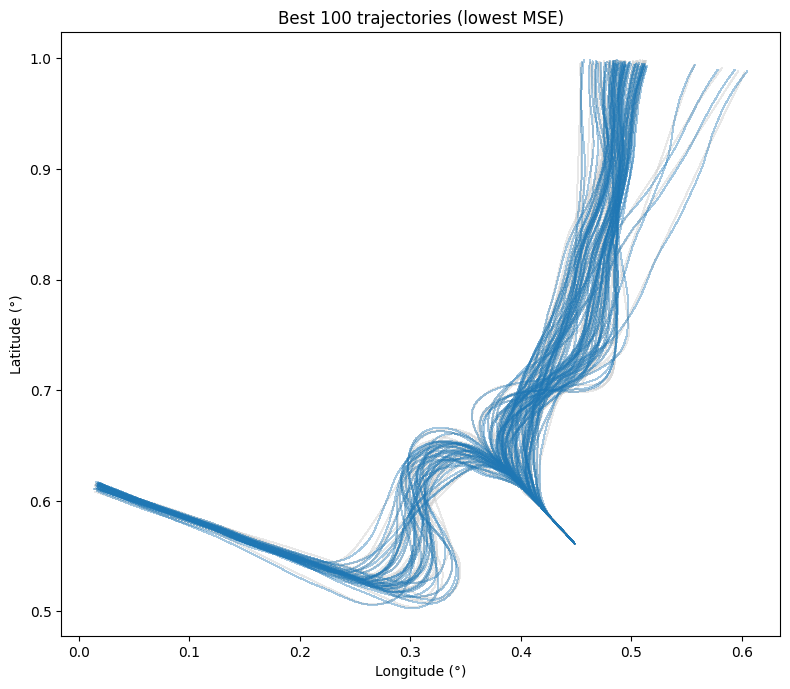
\includegraphics[width=\linewidth, height=4cm, keepaspectratio]{best100}
		}
		{% 标题和标签
			\captionsetup{width=\linewidth} % 让标题宽度匹配图片宽度
			\caption{The best 100 trajectories}
			\label{fig:best100}
		}
		\hfill % 控制两图间距
		
		% --- 右图 ---
		\ffigbox
		[0.45\textwidth]
		{% 图片内容
			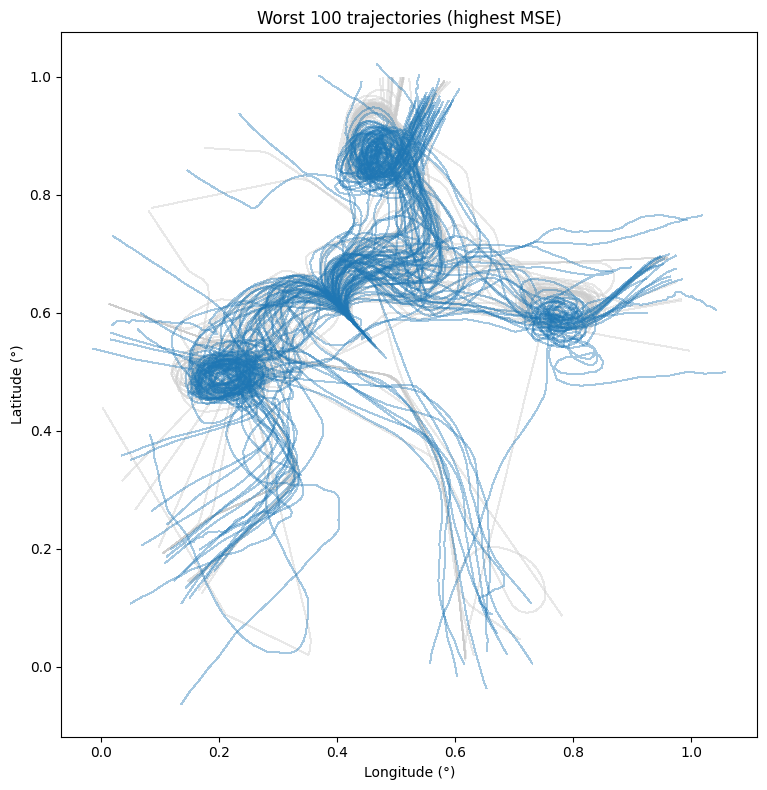
\includegraphics[width=\linewidth, height=4cm, keepaspectratio]{worst100}
		}
		{% 标题和标签
			\captionsetup{width=\linewidth} % 同理,caption 宽度与图相同
			\caption{The worst 100 trajectories}
			\label{fig:worst100}
		}
	\end{floatrow}
\end{figure}

\subsection{Noise Injection}
To systematically analyze the impact of different noise types on AE reconstruction performance, three typical artificial noise sources were injected into the baseline trajectories: Gaussian noise, drift noise, and spike noise. These correspond to the most common sources of error in ADS-B data and collectively simulate disturbances that occur during data acquisition, transmission, and decoding. The experiment procedure is shown in Figure \ref{fig:experiment-structure}.
\begin{figure}[h]
	\centering
	\includegraphics[width=0.6\linewidth]{"experiment structure"}
	\caption{Experimental Flowchart for Evaluating Reconstruction Performance of AE Model}
	\label{fig:experiment-structure}
\end{figure}

Gaussian noise simulates random measurement errors affecting ADS-B signals during reception or localization such as GNSS range errors, multipath propagation, or receiver thermal noise resulting in small position fluctuations. It is implemented by adding Gaussian perturbations to each coordinate dimension of the baseline trajectories.
Drift noise represents time-dependent cumulative deviations caused by positioning or clock synchronization errors, commonly manifested as gradual longitude or latitude shifts over time. This type of error may originate from GNSS reference drift, sensor calibration bias, or timestamp misalignment. It is simulated by superimposing a small linear offset proportional to time on the trajectory coordinates.
Spike noise corresponds to sporadic outliers or sudden jumps in ADS-B messages, such as decoding errors, packet loss, or transient interference leading to abrupt changes in altitude or speed. In the experiment, random subsets of points were selected from each trajectory and perturbed with sudden amplitude changes of random magnitude.
Each of the three noise types was configured with multiple intensity levels to observe how varying magnitudes of error affect model performance. Gaussian noise causes overall jitter while preserving trajectory shape; drift noise induces gradual spatial displacement over time; and spike noise introduces localized abrupt deviations.

The resulting noisy trajectories thus possess controlled and interpretable noise characteristics, closely corresponding to realistic ADS-B error patterns and providing a solid foundation for robustness analysis of the AE model.

\subsection{Metrics and Results}
To quantitatively evaluate the AE model’s reconstruction robustness, the Root Mean Squared Error (RMSE) was adopted as the primary evaluation metric, measuring the overall deviation between the reconstructed and the true noisy trajectories.

For each noise type, experiments were conducted under multiple noise intensity parameters, and the RMSE distribution for each condition was recorded. All tests were performed using the same AE model configuration to ensure that performance variations stem solely from noise perturbations. To enhance statistical reliability, each experiment was repeated 10 times, and the results were averaged.

As shown in Figure \ref{fig:impactofnoise}, the results indicate that:
In the Gaussian noise group, increasing the noise level ($\sigma$) leads to a clear rise in RMSE and greater variance, suggesting high sensitivity to random high-frequency perturbations.
In the drift noise group, RMSE increases slightly with stronger drift, but the overall growth remains slow, indicating that the AE model can capture the global trajectory trend and tolerate gradual cumulative deviations.
In the spike noise group, RMSE shows the smallest fluctuations and remains nearly stable, rising only slightly when the spike probability is high, implying that occasional outliers have limited effect on overall reconstruction.

In summary, the AE model is most sensitive to Gaussian-type random noise, while showing greater tolerance to drift and spike noise. This suggests that, during the ADS-B data cleaning stage, attention should focus on smoothing and reducing high-frequency noise (e.g., localization jitter or measurement fluctuation). In contrast, short-term anomalies or mild drifts can often be mitigated by the model itself. Therefore, noise suppression strategies should emphasize smoothing filters and interpolation optimization, rather than excessive removal of local outliers, in order to preserve the structural integrity of trajectories.

\begin{figure}
	\centering
	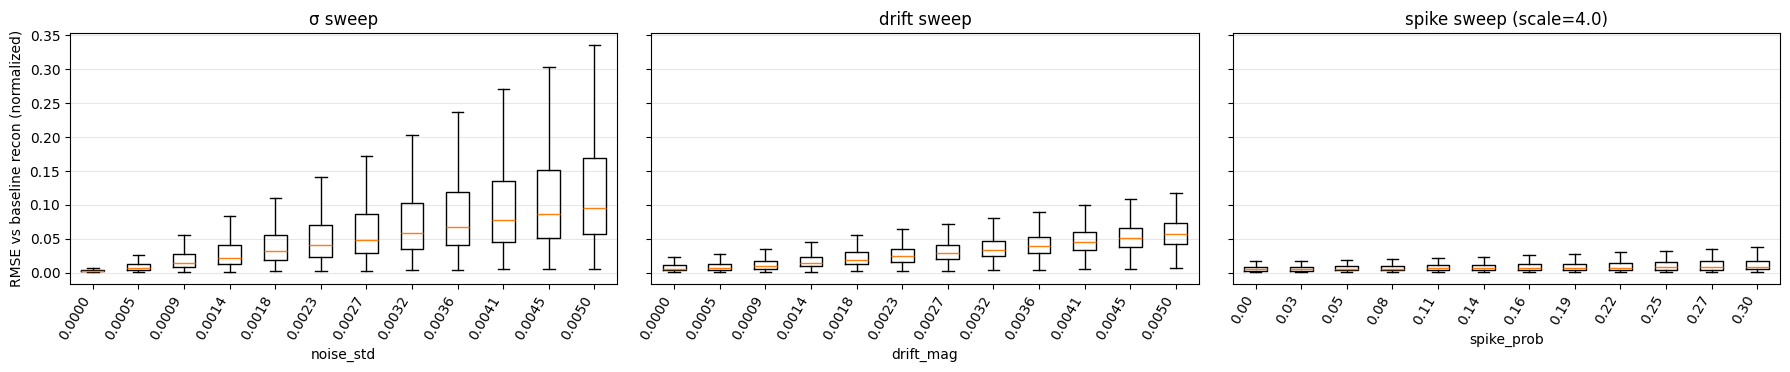
\includegraphics[width=1\linewidth]{impact_of_noise2}
	\caption{Impact of Different Noise Types on AE Reconstruction Performance: Boxplots of Normalized RMSE Between Baseline Reconstruction and Reconstruction of Data with Gaussian Noise ($\sigma$ Sweep), Drift (Drift Sweep), and Spikes (Spike Sweep, Scale=4.0) - N=100 Trajectories, 100 Runs, T=100 Time Steps, Latent Dimension=16}
	\label{fig:impactofnoise}
\end{figure}

\subsection{Discussion}
The choice of the AE as the analytical model was mainly motivated by its simple architecture, unsupervised learning capability, and strong performance in trajectory reconstruction tasks. However, it is important to note that the AE serves only as an illustrative example to reveal the relationship between noise and algorithmic performance. The impact of noise strongly depends on the model’s structure and learning mechanism—models such as LSTM, CNN, or Kalman filters may demonstrate markedly different levels of robustness. Future research will therefore extend the comparative analysis to various model architectures to derive more generalizable conclusions.
Similarly, regarding evaluation metrics, while RMSE effectively measures reconstruction accuracy, additional indicators such as temporal consistency, structural similarity, and feature preservation rate may be introduced in future work to better assess performance in trajectory prediction, classification, or anomaly detection tasks.
Moreover, since the AE model requires a fixed input dimension, this study did not further investigate the effect of missing-value errors on reconstruction performance, which is typically addressed by interpolation or resampling techniques during data cleaning. Future studies can incorporate different data imputation strategies within this framework for comparative analysis.

In conclusion, the experiments and analyses in this chapter validate the AE model’s reconstruction behavior under various noise conditions, providing empirical evidence for understanding how data quality influences algorithmic performance.
Future research will build upon this work by expanding the range of model types, evaluation metrics, and noise modeling complexity, ultimately establishing a comprehensive and interpretable evaluation framework for assessing the impact of ADS-B data cleaning on downstream algorithmic performance.